\documentclass[Analysis-3]{subfiles}
\usepackage{style}

\begin{document}
\chapter*{Lecture 23} %Set chapter name
\addcontentsline{toc}{chapter}{Lecture 23} %Set chapter title
\setcounter{chapter}{23} %Set chapter counter
\setcounter{section}{0}

We will begin this lecture with few examples.
\begin{Eg}{Path Of a Projectile}{}
    \begin{align*}
        \gamma(t)           & =(\alpha t, \beta t-16t^2)               \\
        \implies \gamma'(t) & = (\alpha, \beta -32t)                   \\
        \text{path length}  & = \int \norm{\gamma'(t)}\dd{t}           \\
                            & = \int \sqrt{\alpha^2 +(\beta-32t)^2} dt
    \end{align*}
\end{Eg}

\begin{Eg}{Perimeter of a Circle}{}
    Parametrization of a circle of radius $r$ is given by $\gamma(t) = (r\cos(t),r\sin(t)), t \in [0,2\pi)$.
    \begin{align*}
        \gamma'(t)    & = (-r\sin(t),r\cos(t))                    \\
        \ell (\gamma) & = \int_{0}^{2\pi} \norm{\gamma'(t)}\dd{t} \\
                      & = \int_{0}^{2\pi} r dt                    \\
                      & = 2\pi r
    \end{align*}
\end{Eg}

\begin{Eg}{Arc Length of graph of functions}{}
    Let, $f : [a,b]\to \R$ be a $C^1$ function. Consider $\gamma(t)=(t, f(t))$. It is a smooth curve.
    \begin{align*}
        \gamma'(t)    & = (1,f'(t))                            \\
        \ell (\gamma) & = \int_{a}^{b} \norm{\gamma'(t)}\dd{t} \\
                      & = \int_{a}^{b} \sqrt{1 + f'(t)^2} dt
    \end{align*}
\end{Eg}

\section{Line Integrals}
To integrate a function over a curve we use \textbf{Line integral}. The function we should integrate maybe a \textbf{Scalar Field} or a \textbf{Vector Field}.(A quick example of a Vector Field: $f : \Op{n} \to \R$ be a differentiable function, then $\nabla f$ is a vector field.)

\textbf{Question.} Given a scalar field $f : \Op{n} \to \R$ and $\gamma \equiv c$ be a curve, we want to define $\int_c f$ . But exactly how we can do this?

\textbf{Ans.} $c$ is a curve, so it is bounded subset of $\R^n$. How about thinking of \textbf{Riemann Integration}? For $n \ge 2$, $c$ is \textbf{content zero} in $\R^n$. This does not make any sense! The right way is as following.

\vspace*{0.5cm}

Let, $\gamma :[a,b]\to \R^n$ be a \textbf{Smooth curve}(Or Piecewise Smooth) and $c:= \text{ran}(\gamma)$(on other words path of $\gamma$). Let, $f \in \mathscr{B}(c)$. Given $\mathcal{P} \in \mathscr{P}[a,b]$, $\mathcal{P} : a = t_0<t_1<\cdots <t_m = b$.

\vspace{0.2cm}

\begin{wrapfigure}{r}{0.5\textwidth}
    \centering
    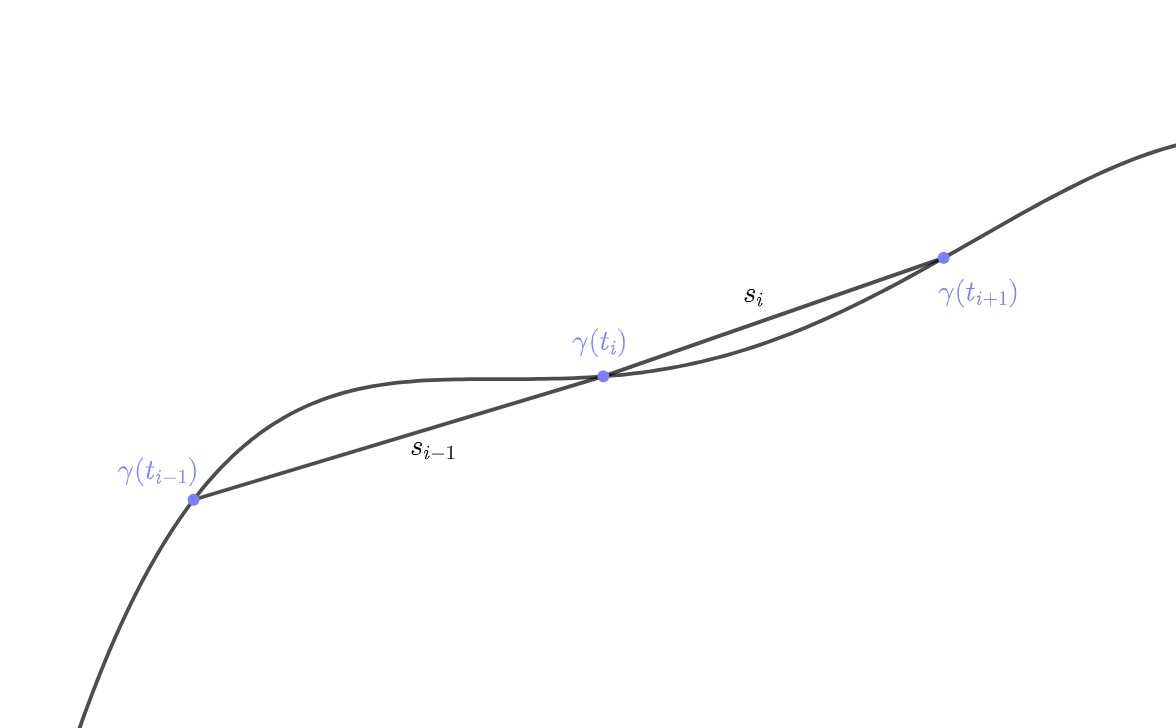
\includegraphics[width=.98\linewidth]{figures/lec-23.1.png}
    \caption{Curve $c$}
\end{wrapfigure}
Let, $I_i = [t_{i-1},t_i]$ be the subintervals and $c_i = \gamma(I_i)$.
Since,$\gamma$ is smooth there is nice correspondence between $I_i$ and $c_i$. Also denote $s_i$ by $\norm{\gamma(t_i) - \gamma(t_i)}$. As previous, define $m_i = \inf_{c_i}f$ and $M_i = \sup_{c_i}f$.
\begin{align*}
    U(f,\mathcal{P}) & = \sum_{i=1}^{m}M_i.s_i \\
    L(f,\mathcal{P}) & = \sum_{i=1}^{m}m_i.s_i
\end{align*}
The above expressions are same as upper and
\vspace{0.05cm}
lower Riemann sum respectively. This opens up ``\textcolor{violet}{The Pandora's box!}''.
\vspace{0.3cm}

$\bullet$ We can now use all the theory we used for the standard Riemann Integrals. We say $f$ is line integrable over $\gamma$ if,
\[\inf_{\mathcal{P} \in \mathscr{P}[a,b]} U(f,\mathcal{P}) = \sup_{\mathcal{P} \in \mathscr{P}[a,b]} L(f,\mathcal{P})\]

More over we will write the common value of the above equality as $\int_c f$ and call this ``The Line Integral over curve $c$''.

\# \textbf{$\mathscr{R}(c)=$} set of all Riemann integrable functions over $c$. Now we can invoke all theory we derived for 1 variable integration!

\begin{Thm}{}{}\label{thm1:23}
    Let, $\gamma$ be a "Rectifiable" smooth(or piecewise smooth) and $c = \text{ran}(\gamma)$ and $f \in \mathscr{B}(c)$. Then,
    \begin{enumerate}
        \item $f \in \mathscr{C} \implies f \in \mathscr{R}(c)$
        \item \[ f \in \mathscr{R}(c) \iff \lim_{||\mathcal{P}||\to 0} \sum_{i=1}^{m} f(\zeta_i)s_i \hspace{0.1cm} \text{exist and equal to}\int_c f.\] Here, $\zeta_i$ is tag of the interval $I_i$.

        \item (This requires smoothness) If $\gamma$ is $C^1$ and smooth , $f \in \mathscr{R}(c)$, then
              \[\int_c f = \int_a^b f(\gamma(t))\norm{\gamma'(t)} \label{eq:1}\]

    \end{enumerate}
\end{Thm}

\textit{Proof.} \textbf{Homework}.

\vspace{0.2cm}

In the above theorem equation in \ref{eq:1} is also independent of choice of Parametrization of $\gamma$. Because any other smooth parametrized curve $\tilde{\gamma} = \gamma \circ \varphi$ where, $\varphi$ is an onto continuous function.

\vspace{1cm}

\textbf{\underline{Facts:}} $c$ be a piecewise smooth, parametrized curve $\gamma$. $f,g \in \mathscr{R}(c)$ and $r \in \R$,then
\begin{itemize}
    \item $\int f+rg = \int f + r\int g $
    \item $f \ge g$ over $c$ then $\int f \ge \int g$
    \item $\int \abs{f} \ge \abs{\int f}$
    \item If $a<d<b$, if $\gamma_1 := \gamma |_{[a,d]}$ and $\gamma_2 := \gamma |_{[d,b]}$ then
          \[\int_c f = \int_{\gamma_1}f + \int_{\gamma_2} f \]
\end{itemize}

We have resolved the problems for Scalar field.\textbf{ What about vector fields ?}
\begin{figure}[H]
    \centering
    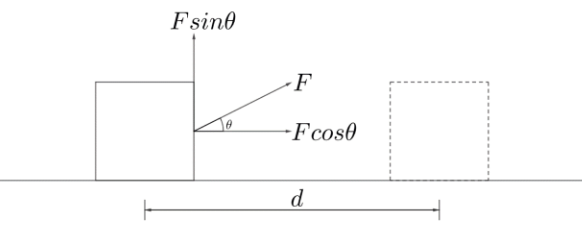
\includegraphics[width=0.5\textwidth]{figures/lec-23.2.png}
    \caption{Work done by a constant Force}
\end{figure}
Suppose a particle moves a distance $d$ under a constant force $F$, then work done by the force is $Fd\cos{\theta} = \vec{F}\cdot\vec{d}$.


\begin{wrapfigure}{r}{0.5\textwidth}
    \centering
    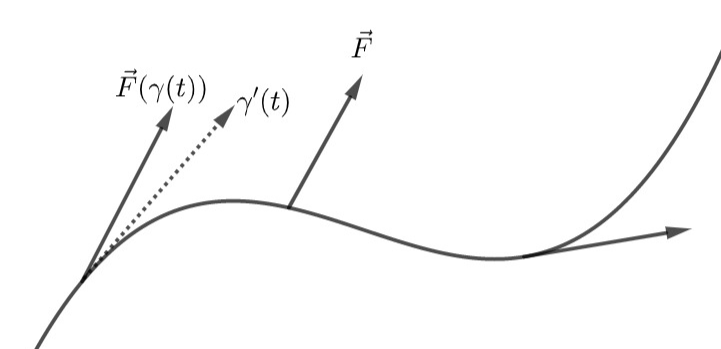
\includegraphics[width=.98\linewidth]{figures/lec-23.3.png}
    \caption{$\vec{F}$ is the vector field over the curve $\gamma$}
\end{wrapfigure}

If the force was not constant throughout the path then how can we calculate work done by that force?
Consider the case where $F$ is the vector field (Force in this case) defined over a curve (path)$\gamma$. Here, $\gamma : [a,b] \to \R^n$ and $c = \text{ran}(\gamma)$. So, work done throughout the whole path will be,
\[\int_c \vec{F}\cdot d\vec{r}\]
Which is equal to, $\int_a^b \vec{F}(\gamma(t))\cdot \nabla \gamma(t) dt$

Now we will look into some examples.
\vspace{0.3cm}

\textbf{Example} 23.1.1  Find work done by the field $F(x,y,z) = (xy,xz,yz)$ along the curve $\gamma(t) = (t^2,-t^3,t^4),t \in [0,1]$.

\textit{Ans.} \begin{align*}
    \gamma'(t)               & = (2t,-3t^2,4t^3)                                 \\
    \implies \text{workdone} & = \int_0^1 (-t^5,t^6,-t^7)\cdot(2t,-3t^2,4t^3) dt \\
                             & = -\frac{31}{88}
\end{align*}

\begin{center}
    \large \underline{\textbf{Line Integration of a Vector Field} }
\end{center}

$F:\Op{n} \to \R^n$ be a vector field and $\gamma:[a,b] \to \Op{n}$ be a curve. We consider a partition $\mathcal{P}: a =t_0<t_1<\cdots < t_m=b$, Let $c_i = \gamma|_{[t_{i-1},t_i]}$ and $\gamma_i = \gamma(t_i)$, $\Delta r_i = \gamma_{i} - \gamma_{i-1}$.
\[R(F;\mathcal{P})= \sum_{i=1}^m F(\gamma_i)\cdot \Delta r_i\]
\begin{align*}
    \int_c \vec{F}\cdot d\vec{r} = \lim_{\norm{\mathcal{P}}\to 0} R(F,\mathcal{P}) \tag{if the limit exists}
\end{align*}
Just like the scalar field, if $\gamma$ is $C^1$ and smooth, then
\[\int_c \vec{F}\cdot d\vec{r} = \int_a^b F(\gamma(t))\cdot \gamma'(t) dt \label{eq:3} \cdots (\ref{eq:3})\]


\end{document}